\section{Asservissement en position de l'UAV}

\subsection{Présentation du contrôleur}

Les équations dynamiques définissant l’évolution d’un quadrotor sont connues \footnote{\url{https://www.wilselby.com/research/arducopter/modeling/}} \cite{uavequation}. C’est pourquoi il est facile de simuler le comportement de ce robot. 
Nous choisirons ici de commander le drone sans se préoccuper de sa dynamique, 
c'est-à-dire que l’on va le contrôler en s’inspirant de la manière dont un pilote pourrait le faire.


On va donc devoir implémenter un contrôleur, qui en connaissant une position voulue pour le drone et sa position actuelle, 
va trouver les commandes à lui appliquer afin de l'amener dans cet état souhaité. Cette méthode de type (PID) présente 
l’avantage de ne pas avoir besoin de manipuler les équations d’état d’un quadrotor qui peuvent être compliquées, 
bien que connues, afin d’établir les commandes à lui appliquer. On aurait pu à ce titre utiliser une méthode de bouclage linéarisant. 
On verra que les résultats produits par notre méthode sont tout de même satisfaisants.

Nous devons donner à notre PID un vecteur vitesse désiré. 
Ce vecteur vitesse est calculé en phase d’approche par la méthode des potentiels artificiels \cite{Khatib}. 
Il s’agit d’une analogie avec l’électromagnétisme. On considère la position souhaitée comme une charge électrique fictive 
produisant un champ électrique dans son voisinage nommé $ E = \nabla v $ 

puis on peut alors déterminer la force à  appliquer au quadrotor qui est proportionnelle au champ électrique. 
Nous devons donc aligner le vecteur vitesse du drone avec le vecteur de force du champ de potentiel. Notre drone sera donc asservi en vitesse, 
quelle que soit la force demandée le drone doit être capable d’aligner son vecteur vitesse avec la force. 

\subsection{Asservissement en vitesse de l'UAV}
On effectue l’asservissement en plusieurs étapes, pour rendre le vecteur vitesse et le vecteur force colinéaires entre eux. 
D’abord, on place le vecteur force dans le repère du drone. Puis on le projette sur le plan $XY$, on calcule l’angle $\Psi$ de lacet et 
on exécute un contrôleur de type PID \ref{fig:pid} pour déplacer en lacet d’un angle $\Psi$ le drone. 
Nous effectuons la même chose pour l’angle de tangage $\theta$, que l’on obtient en projetant sur l’axe $ZY$. 
A la fin de ces actions, le vecteur force fourni par le champ de vecteurs est confondu avec l’axe $X$ 
support du roulis du drone. Finalement les actions effectuées par l’algorithme sont très semblables 
à ce que peut faire le pilote de drone avec sa télécommande permettant de commander le tangage et le lacet du drone, 
mais c’est l'oeil qui estime l’état et calcule l’erreur pour déterminer les bonnes actions en sortie. 

\begin{figure}[!htb]
    \centering
    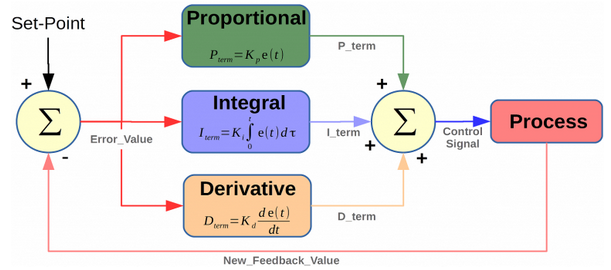
\includegraphics[width=0.7\textwidth]{./asservissement_drone/pid.png}
    \caption{Contrôleur PID sur $\Psi$ et $\theta$}
    \label{fig:pid}
\end{figure}


\begin{figure}[!htb]
    \centering
    \begin{subfigure}[b]{0.4\textwidth}
        \centering
        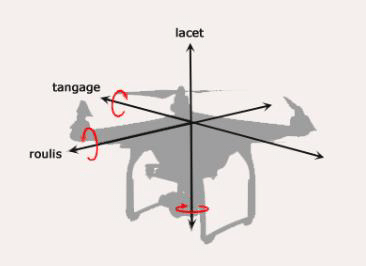
\includegraphics[width=\textwidth]{./asservissement_drone/drone_schema.png}
        \caption{Schema de fonctionnement du drone}
        \label{fig:marker}
    \end{subfigure}
    \hfill
    \begin{subfigure}[b]{0.4\textwidth}
        \centering
        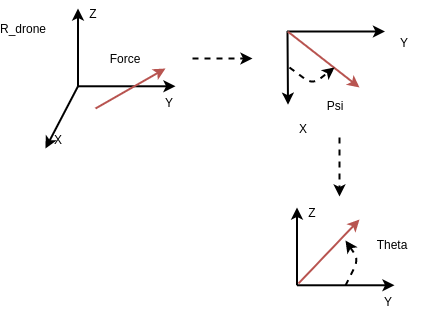
\includegraphics[width=\textwidth]{./asservissement_drone/projection.png}
        \caption{Asservissement en vitesse du drone}
        \label{fig:manifold}
    \end{subfigure}
    \caption{Schema de fonctionnement du contrôleur}
    \label{fig:environnement}
\end{figure}

\section{Résultats}

Nous avons donc mis en place l’idée précédente et utilisé le contrôleur cmd\_vel
du package hector\_quadrotor qui effectue le contrôleur PID décrit avant et permet d’asservir l’UAV en vitesse.
Sur les figures ci-dessous, on peut voir la trajectoire elliptique du marker dans l’espace 3D ainsi que 
l’évolution de la distance entre le marker et l’UAV au cours du temps. 
On remarque qu’au bout d’une dizaine de secondes l’UAV se place à une distance de moins de 5 m. 
Le contrôleur est satisfaisant. \footnote{\url{https://github.com/ENSTA-Bretagne-Autoland-2021/high-level-commands/blob/main/src/vel_node.py}}

\begin{figure}[!htb]
    \centering
    \begin{subfigure}[b]{0.4\textwidth}
        \centering
        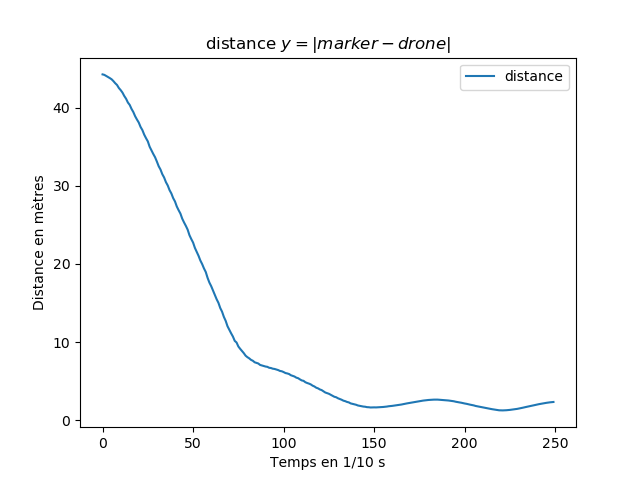
\includegraphics[width=\textwidth]{./asservissement_drone/convergence.png}
        \caption{Distance au de l'UAV Hector au Marker}
        \label{fig:convergence}
    \end{subfigure}
    \hfill
    \begin{subfigure}[b]{0.5\textwidth}
        \centering
        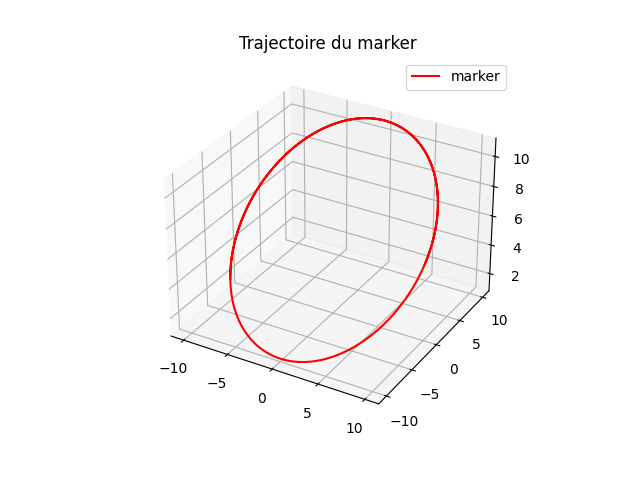
\includegraphics[width=\textwidth]{./asservissement_drone/marker.png}
        \caption{Ellispe parcourue par l'UAV}
        \label{fig:manifold}
    \end{subfigure}
    \caption{Résultats de la simulation}
    \label{fig:ellipse}
\end{figure}